%\documentclass[draft]{agujournal2018}
\documentclass[]{agujournal2018}
\usepackage{apacite}
\usepackage{url}
\usepackage{lineno}
%\linenumbers
\draftfalse
\journalname{Geophysical Research Letters}

%custom packages
\usepackage{amsmath,amssymb,amsfonts,amsthm}
\usepackage{comment}
\usepackage{booktabs}
% custom commands
\newcommand\be{\begin{equation}}
\newcommand\ee{\end{equation}} 
\newcommand\bra{\langle}
\newcommand\ket{\rangle}
\newcommand\om{\omega}
\newcommand\tom{\tilde{\omega}}
\newcommand\tg{\tilde{g}}
\newcommand\tp{\tilde{p}}
\newcommand\tG{\tilde{G}}
\newcommand\El{\mathcal{L}}

\begin{document}

\title{Back to Einstein: how to include burial in fluvial sediment diffusion models?}

\authors{James K. Pierce \affil{1}and Marwan A. Hassan\affil{1}}
\affiliation{1}{Department of Geography \\University of British Columbia}
\correspondingauthor{James Kevin Pierce}{kpierce@alumni.ubc.ca}

\begin{keypoints}
\item We develop a random-walk model of objects in intermittent transport through an environment with traps.
\item Its solution provides three ranges of diffusion, two of which are anomalous.
\item We apply the model transported sediment undergoing burial within a river channel and clarify the scale-dependence of bedload diffusion.

\end{keypoints}

\begin{abstract}
	

In gravel-bed rivers, grains move through a sequence of motions and rests. 
Differences in the movement characteristics of one grain and the next imply sediment diffusion, whereby individual grains spread apart as they transport.
When grains rest on the surface, they can be buried by material transported from upstream.
Buried grains are not exposed to the fluid flow, so these grains are immobile for relatively long periods, only being mobile again once they're uncovered.  This crucially modifies the diffusion characteristics of transported sediment.
Despite the importance of sediment burial to diffusion, very few diffusion models have accounted for it.
In this letter, we develop a random-walk model to incorporate sediment burial.
The model predicts three ranges of sediment diffusion with distinct characteristics in each range.
We express the crossover times between these ranges in terms of measurable transport parameters, and explain each range in terms of underlying physical processes.
This provides new geophysical understanding of the scale-dependent phenomenon of fluvial sediment transport. 
Understanding the multiple ranges of sediment diffusion in river channels will improve predictions of channel morphodynamics.
\end{abstract}

\section{Introduction}
% what is problem and why does it matter
Anomalous diffusion has been the topic of intense study, since it appears in contexts as diverse and important as the transport of cholesterols through lipid bilayers \citep{Jeon2012,Molina-Garcia2018}, contaminants through soils \citep{Berkowitz2006,Yang2019}, and pollinator insects through ecosystems \citep{Reynolds2009,Vallaeys2017}.
Emerging research in fluvial geomorphology has found its way to anomalous diffusion as well, since coarse sediment grains transporting through river channels apparently display it \citep{Martin2012,Bradley2017}.
\citet{Einstein1937} developed the first model of fluvial bedload diffusion, which is the spreading apart of grains as they transport downstream.
Diffusion is induced by differences in the transport characteristics of one grain and the next, and it is usually quantified by the time-dependence of the positional variance $\sigma_x^2(t)$ of a population.
When $\sigma_x^2 \propto t$, the diffusion is said to be normal, since this is found in the classic diffusion problems \citep[e.g.][]{Einstein1905,Taylor1920}.
However, many transport phenomena show $\sigma_x^2 \propto t^\gamma$, with $\gamma \neq 1$. This diffusion is said to be anomalous \citep{Sokolov2012}.
If $\gamma>1$, it is said to be super-diffusive; while if $\gamma <1$, it is said to be sub-diffusive \citep{Metzler2000}.

% what do we know about it 
Since Einstein, investigators have come to recognize that coarse sediment moving through river channels can show either anomalous or normal diffusion depending on the timescale of observation \citep{Nikora2002}.
This is a significant issue since it implies diffusion models should be scale dependent, and it renders experimental data contingent on their observation timescales.
\citet{Nikora2001a,Nikora2002} first identified three ranges of bedload diffusion from simulations and experimental data, and they termed these local, intermediate, and global ranges in order of increasing scale.
$\sigma_x^2$ scales with time differently in each range, and this scaling can be anomalous or normal.
Their findings are supported by a wide set of contemporary data and numerical simulations that show up to three ranges of bedload diffusion \citep{Martin2012, Bialik2012, Zhang2012, Fan2016, Bradley2017,Wu2019}.
While earlier works have developed models of bedload diffusion, there are contradictions in the literature about the expected diffusion characteristics (super/normal/sub-diffusion) of each range, and no model has been developed, to our knowledge, that derives all three diffusion ranges from process-based concepts of fluvial sediment transport.

% how do we approach it
In this letter, we present a model of bedload diffusion which describes local, intermediate, and global ranges by including the duration of motion and the possibility of trapping due to burial into the classic bedload diffusion model of \citet{Einstein1937}.
Einstein's model has been highly influential in river geophysics and has fostered an entire paradigm of research that leverages and generalizes his stochastic methods \citep[e.g.][]{Hubbell1964, Yano1969, Yang1971, Gordon1972, Nakagawa1976}.
Its essential content is that individual grains move in instantaneous steps interrupted by durations of rest which lie on statistical distributions \citep{Hassan1991}.
It predicts a single range of normal diffusion \citep{Einstein1937, Nakagawa1976}.
Essentially, the Einstein model is a special case of the continuous time random walk (CTRW) \citep{Montroll1965}, originally developed to describe anomalous diffusion of charge carriers in solids.
To include the duration of motion and the burial process we leverage the multi-state generalization of the CTRW developed by \citet{Weiss1976, Weiss1994}.
Our development allows us to derive three ranges of diffusion and the scaling behavior of $\sigma_x^2$ in each range. The model is analytically solvable, and we determine the cross-over times between diffusion ranges.
Several progressive works have discriminated multiple ranges of bedload diffusion due to the duration of motion \citep{Lisle1998} and sediment burial \citep{Wu2019}, and multiple ranges of diffusion have been shown in models of other transport phenomena \cite[e.g.][]{Bena2006, Balakrishnan1988, Flekkøy2017, AaraoReis2014}.
However, we believe our proposed model is the first analytically solvable model of three diffusion ranges.
We present the model in section \ref{sec:model} and solve it in section \ref{sec:solution}.
We use the solution in section \ref{sec:discussion} to directly attribute physical processes to each diffusion range, to discern the crossover times between ranges in terms of empirically measurable transport parameters, and to derive earlier works as limiting cases \citep[e.g.][]{Lisle1998,Wu2019,Einstein1937}.

\section{Bedload diffusion with burial as a multi-state random walk}
\label{sec:model}
We use a three-state random walk where the states are motion, rest, and burial.
We label these as $i=2$ (motion), $i=1$ (rest), and $i=0$ (burial).
Our development of the governing equations for the three-state walk closely mimics \citet{Weiss1994}, and our approach to incorporating the trapping process closely mirrors \citet{Schmidt2007}. 
In our model, residence times in motion and rest states are random variables characterized by exponential distributions and motions are characterized by a constant velocity $v$.
We consider burial to be a permanent condition which has some probability to occur when resting grains are covered by transported sediment.
The probability of burial per unit time (burial rate) is considered constant, so the probability of trapping increases with the time grains spend resting.

% describe meaning of sojourns and g_i/G_i/theta_i
A central concept in our derivation is the idea of a sojourn in the state $i$ \citep{Weiss1994}.
When a grain enters a state $i$ at some time $t_0$ and position $x_0$, then leaves a state at some other time $t_1$ and position $x_1$, we say that the grain has completed a sojourn in the state $i$. The joint probability density for a complete sojourn through the state $i$ of time $\tau = t_1-t_0$ and displacement $\xi = x_1-x_0$ is denoted $g_i(\xi,\tau).$ Similarly, we can consider incomplete sojourns. If a grain begins a sojourn in the state $i$ at $(t_0,x_0)$ and the sojourn is still on-going, the joint probability density to find the grain at $(x_1,t_1)$ is $G_i(\xi,\tau)$. The $g_i$ and $G_i$ can be further decomposed when time and space components of the motion are independent \citep{Weiss1994}.
We refer to $g_i$ and $G_i$ as the complete and incomplete propagators, since they move probability through space-time and are associated respectively with complete and incomplete sojourns.

% discuss two-stage derivation of weiss
Our target is the probability distribution $p(x,t)$ to find a grain at $x,t$ if we know it started at $(x,t)=(0,0)$, i.e., with the initial distribution $p(x,0)=\delta(x)$.
We denote the initial probabilities to be at rest or in motion as $\theta_1$ and $\theta_2$. 
Normalization requires $\theta_1+\theta_2=1$.
Our derivation has two main steps.
First, we introduce and solve for a set of joint probabilities associated with transitions of a grain from one state to another.
Second, we use these quantities to solve for the probabilities that a grain is in state $i$ having position $x$ at time $t$.
Afterward, we sum the these distributions over all states $i$ to derive the joint probability that a grain is in any state at $(x,t)$.

% derive omegas
Now we begin the first stage of the derivation.
Grains at rest may be trapped by burial.
We consider burial to be permanent \citep[e.g.][]{Wu2019}, and we assume resting grains may be buried with constant probability per unit time $\kappa$.
From this assumption, the probability that a grain is not trapped after a time $t$ at rest is given by a survival probability $\Phi_F(t) = e^{-\kappa t}$ ($F$ is for "free"). Likewise, the probability that it is trapped after resting for a time $t$ is the complement $\Phi_T(t) = 1-\Phi_F(t)$ ($T$ is for "trapped").
We introduce $\omega_{1T}(x,t)$, $\omega_{1F}(x,t)$, and $\omega_2(x,t)$ as the joint probabilities to find a grain at $(x,t)$ having just completed a sojourn.
The subscript ${1T}$ denotes the completion of a rest sojourn due to trapping by burial, while $1F$ denotes the completion of a rest sojourn due to motion.
Similarly, the subscript $2$ denotes the completion of a motion sojourn due to the onset of resting.
Using an argument similar to \citet{Weiss1994}, we write integral equations to link the $\omega$'s: 
\begin{align}
\om_{1T}(x,t) &= \theta_1\Phi_T(t)g_1(x,t) + \int_0^x dx' \int_0^t dt' \om_2(x',t')\Phi_T(t-t')g_1(x-x',t-t')\label{eq:x}\\
\om_{1F}(x,t) &= \theta_1\Phi_F(t)g_1(x,t) + \int_0^x dx' \int_0^t dt' \om_2(x',t') \Phi_F(t-t') g_1(x-x',t-t')\\
\om_2(x,t) &= \theta_2 g_2(x,t) + \int_0^x dx' \int_0^t dt' \om_{1F}(x',t')g_2(x-x',t-t') \label{eq:y}
\end{align}
The first equation can be understood as follows: $\omega_{1T}(x,t)$ describes the probability that a sojourn in the state $1$ ends due to trapping at $(x,t)$. This quantity has two contributions. The first contribution represents the possibility that the grain started at $(x,t)=(0,0)$ in the $i=1$ state (with probability $\theta_1$), propagated a distance $x$ and a time $t$ in the $i=1$ state (with probability $g_1(x,t)$), was trapped (with probability $\Phi_T(t)$), and is now at $(x,t)$. 
The second contribution describes the possibility that the grain was in a motion sojourn which ended at $x',t'$ when it came to rest. From here, it propagated from $x',t'$ to $x,t$ at rest (with probability $g_1(x-x',t-t')$) and was trapped during this sojourn (with probability $\Phi_T(t-t')$).
The other equations can be reasoned similarly; these arguments are analogous to \citet{Weiss1994}.
Once the propagators are specified, we can solve (\ref{eq:x}-\ref{eq:y}) for the $\omega$'s. This completes the first stage of the derivation.

% derive p's
The second stage of our derivation involves the joint probabilities of being in state regardless of whether a sojourn has just completed. These are denoted by  $p_0(x,t)$ (trapped), $p_1(x,t)$ (rest), and $p_2(x,t)$ (motion), and they involve the $\omega$'s for their definition:
\begin{align}
p_0(x,t) &= \int_0^t dt' \omega_{1T}(x,t-t') \label{eq:b}\\
p_1(x,t) &= \theta_1 G_1(x,t) + \int_0^x dx' \int_0^t dt' \omega_2(x',t')G_1(x-x',t-t')\label{eq:a}\\
p_2(x,t) &= \theta_2 G_2(x,t) + \int_0^x dx' \int_0^t dt'  \omega_{1F}(x',t')G_2(x-x',t-t').\label{eq:z}
\end{align}
Equation (\ref{eq:b}) says that grains buried at any $(x,t)$ arrived there due to trapping at $x$ at any time leading up to $t$.
The reasoning in (\ref{eq:a}-\ref{eq:z}) is the same as for (\ref{eq:x}-\ref{eq:y}), except we use the propagators for incomplete sojourns.
These equations can be solved once the propagators are specified and the $\omega$'s are known from (\ref{eq:x}-\ref{eq:y}).
Finally, we form the total probability density for a grain to be found at $(x,t)$ in any state.
This is simply 
\be p(x,t) = p_0(x,t) + p_1(x,t) + p_2(x,t). \label{eq:dist}\ee
This joint density is completely determined once (\ref{eq:x}-\ref{eq:z}) are solved.


\section{Specification of propagators and solution of model}
\label{sec:solution}
% choice of propagators
We consider sojourns in the rest state to occur for an exponentially distributed time interval, given by the distribution $\psi_1(t) = k_1 e^{-k_1t}.$
The probability that a sojourn in this state lasts for at least the time $t$ is then given by $\Psi_1(t) = \int_t^\infty \psi_1(t)dt = e^{-k_1 t}$.
Since resting grains do not move, the probability of finding the grain at its starting position is $1$, while the probability of finding it anywhere else is zero.
Hence the complete propagator for a rest sojourn is $g_1(x,t) = \delta(x)\psi_1(t),$ or 
\be g_1(x,t) = \delta(x)k_1e^{-k_1t}.\label{eq:prop1} \ee
Likewise, the incomplete propagator for a rest sojourn is $G_1(x,t) = \delta(x)e^{-k_1t} = g_1(x,t)/k_1.$
The motion propagators are reasoned similarly.
We consider motions to occur with a constant velocity $v$ and to have an exponentially distributed duration given by $\psi_2(t) = k_2 e^{-k_2t}.$
Since motions are considered deterministic, the probability to find a grain at position $x$ in a motion sojourn is $\delta(x-vt)$, and the complete propagator is 
\be g_2(x,t) = \delta(x-vt)k_2e^{-k_2t},\label{eq:prop2}\ee
while the incomplete propagator is $G_2(x,t) = g_2(x,t)/k_2$ as before.

% distribution functions and moments in laplace space
Having defined the propagators, we set out to solve (\ref{eq:x}-\ref{eq:z}) and understand bedload diffusion with a finite motion interval and when subject to trapping by burial.
The convolution structure of (\ref{eq:x}-\ref{eq:z}) presents a formidable problem.
Luckily, we have the device of Laplace transforms.
These project integro-differential equations into an alternate space in which convolutions are unraveled \citep[e.g.][]{Arfken1985}.
The double Laplace transform of a joint probability distribution $p(x,t)$ is defined by 
\be \tilde{p}(\eta,s) = \int_0^\infty dx e^{-\eta x}\int_0^\infty dt e^{-st} p(x,t) \label{eq:doubletransform}\ee
The Laplace-transformed moments of $x$ are linked to derivatives of the double-transformed distribution.
From (\ref{eq:doubletransform}) it's clear that
\be \bra \tilde{x}(s)^k \ket = (-)^k\partial_\eta^k p(\eta,s)\Big|_{\eta=0}.\label{eq:momenttrick}\ee
The operator $\bra \circ \ket$ denotes the ensemble average \citep[e.g.][]{Kittel1958}.
This means we can compute the variance of position as $\sigma_x^2(t) = \bra x^2 \ket - \bra x \ket^2 = \El^{-1} \{\bra\tilde{x}^2 \ket;t\} - \El^{-1} \{\bra\tilde{x} \ket;t\}^2$, where $\El^{-1}$ denotes the inverse Laplace transform \citep[e.g.][]{Arfken1985}. This is a powerful tool, since we can use it to derive the positional variance without integrating the distribution in equation (\ref{eq:dist}).


% solution for case theta_1=1: distribution function
Using the propagators (\ref{eq:prop1}-\ref{eq:prop2}) and this transform calculus, the joint distribution $p(x,t)$ is derived in appendix \ref{sec:appendixA}, while the moments $\bra x \ket$ and $\bra x^2 \ket$, and ultimately the variance of position $\sigma_x^2(t)$, are derived in appendix \ref{sec:appendixB}. Using the shorthand notation $\xi = k_2 x/v$ and $\tau = k_1(t-x/v)$ \citep[c.f.][]{Lisle1998} and assuming all grains start from motion ($\theta_1=1$), the distribution is 
\begin{multline}
p(x,t) = e^{-(\kappa + k_1)\tau/k_1-\xi}\mathcal{H}(\tau)\mathcal{H}(\xi)\Bigg[\frac{k_1}{v}\delta(\tau) + \frac{k_1}{v} \sqrt{\frac{\xi}{\tau}}\mathcal{I}_1(2\sqrt{\xi\tau}) + \frac{k_2}{v} \mathcal{I}_0(2\sqrt{\xi\tau})\Bigg]\\
+ \kappa \frac{k_2}{v(\kappa+k_1)}\mathcal{H}(\tau)\mathcal{H}(\xi)e^{-\xi}\mathcal{P}_1\big(\kappa\xi/(\kappa+k_1), (\kappa+k_1)\tau/k_1\big).
\label{eq:pdf}
\end{multline}
The $\mathcal{I}_\nu$ are modified Bessel functions of the first kind and $\mathcal{P}_1$ is a (complementary) Marcum Q-function defined by $\mathcal{P}_1(x,y) = \int_0^y e^{-z-x}\mathcal{I}_0(2\sqrt{xz})dz $ \citep{Temme1996}. The Q-function was initially introduced in relation to radar detection theory \citep{Marcum1960}. $\mathcal{H}(x)$ is the Heaviside step function and we use the convention $\mathcal{H}(0)=1$.
The distribution (\ref{eq:pdf}) is depicted in figure \ref{fig:pdfs}.

% figure showing distribution functon
\begin{figure}
	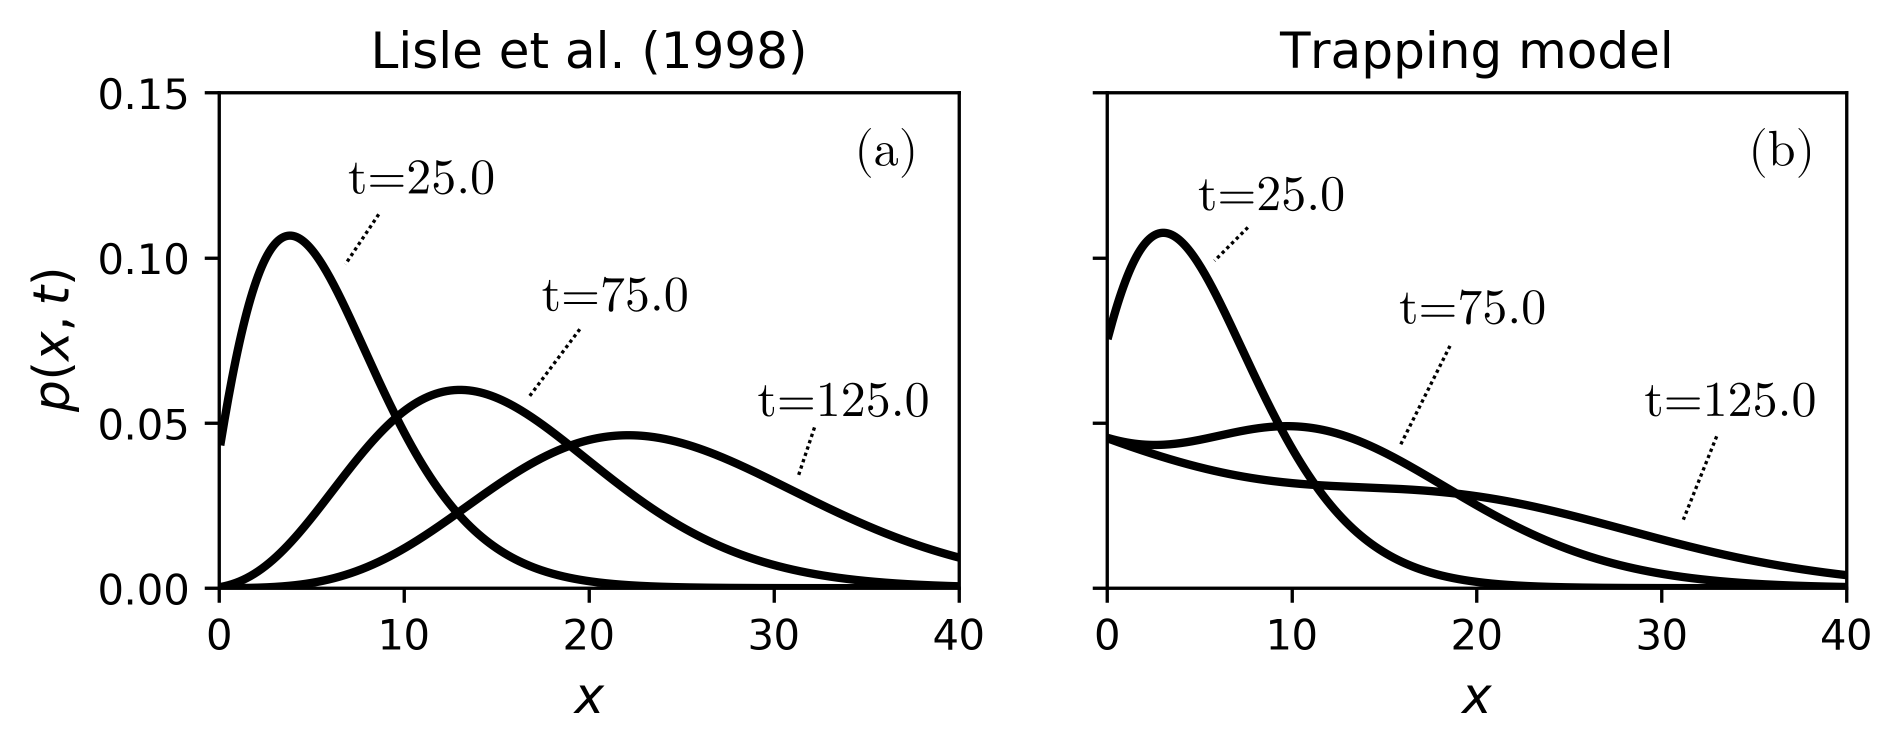
\includegraphics[width=\linewidth,keepaspectratio]{./figures/pdf-plot-edit.png}
	\caption{Joint distributions of a tracer being found at $x$ $t$ are impeded by the trapping process. Panel (a) shows the \citet{Lisle1998} model, and panel (b) shows the the distribution \ref{eq:pdf} which results from a trapping process occurring at rate $\kappa$. Cross-comparison of both panels shows that trapping redistributes probability to smaller values of $x$, and this redistribution becomes more important for larger $t$.}
	\label{fig:pdfs}
\end{figure}
% solution for theta_1=1: moments
\noindent The first two moments are
\be \bra x(t) \ket = A_1 e^{(b-a)t}+B_1e^{-(a+b)t}+C_1 \label{eq:mean}\ee
\be \bra x^2(t) \ket = A_2(t)e^{(b-a)t}+B_2(t)e^{-(a+b)t}+C_2. \label{eq:second}\ee

The $A_i$ and $B_i$ are polynomials available in table (\ref{table:params}).
In terms of these moments, the variance is
\be \sigma_x^2(t) = A(t)e^{(b-a)t} + B(t)e^{-(a+b)t} + C(t) \label{eq:var}\ee
Where $A, B,$ and $C$ are transcendental functions in table in (\ref{table:params}).
We have made no approximation to derive this expression.
It represents the downstream diffusion of bedload grains when motion durations and the possibility of burial within the sedimentary bed are accounted for.
\begin{table}[!h]
	\centering
	\caption{Polynomials and transcendental functions used in the expressions of the mean (\ref{eq:mean}), second moment (\ref{eq:second}) and variance (\ref{eq:var}) of bedload tracers.}
	\label{table:params}
	\begin{tabular}{c}
		\toprule
		$A_1 = \frac{v}{2b}\big[1+\frac{\kappa+k_1}{b-a}\big]$ \\
		$B_1 = -\frac{v}{2b}\big[1-\frac{\kappa+k_1}{a+b}\big]$ \\
		$C_1 =  -\frac{v}{2b}\big[\frac{\kappa+k_1}{b-a}+\frac{\kappa+k_1}{a+b}\big]$\\
		$A_2(t)=\frac{v^2}{2b^3}\Big[b+(b-a)[bt-1]+2(\kappa+k_1)[bt-1] + \frac{(\kappa+k_1)^2}{(a-b)^2}[-abt+a+b(bt-2)]\Big] $\\
		$B_2(t) = \frac{v^2}{2b^3}\Big[b-(a+b)[bt+1]+2(\kappa+k_1)[bt+1] - \frac{(\kappa+k_1)^2}{(a+b)^2}[bt(a+b)+a+2b]\Big] $\\
		$C_2(t) = \frac{v^2}{2b^3}(\kappa+k_1)^2\Big[\frac{a+2b}{(a+b)^2}+\frac{-a+2b}{(a-b)^2}\Big]$\\
		$A(t) = A_2(t)-2A_1C_1 + A_1^2\exp[(b-a)t]$\\
		$B(t) = B_2(t)-2B_1C_1 + B_1^2\exp[-(a+b)t]$\\
		$C(t) = C_2(t)-C_1^2+2A_1B_1\exp[-2at]$\\
		\bottomrule
	\end{tabular}
\end{table}




\section{Discussion: new findings and foundational links}
\label{sec:discussion}

\subsection{bedload diffusion}
% plot variance
A plot of $\sigma_x^2(t)$ is shown in figure \ref{fig:var} for the case that motions are short relative to rests, and trapping occurs with characteristic timescale $1/\kappa$ which is in turn much shorter than the resting period.
That is, for the case that $1/k_2 \ll 1/k_1 \ll 1/\kappa$.
\begin{figure}[t]
	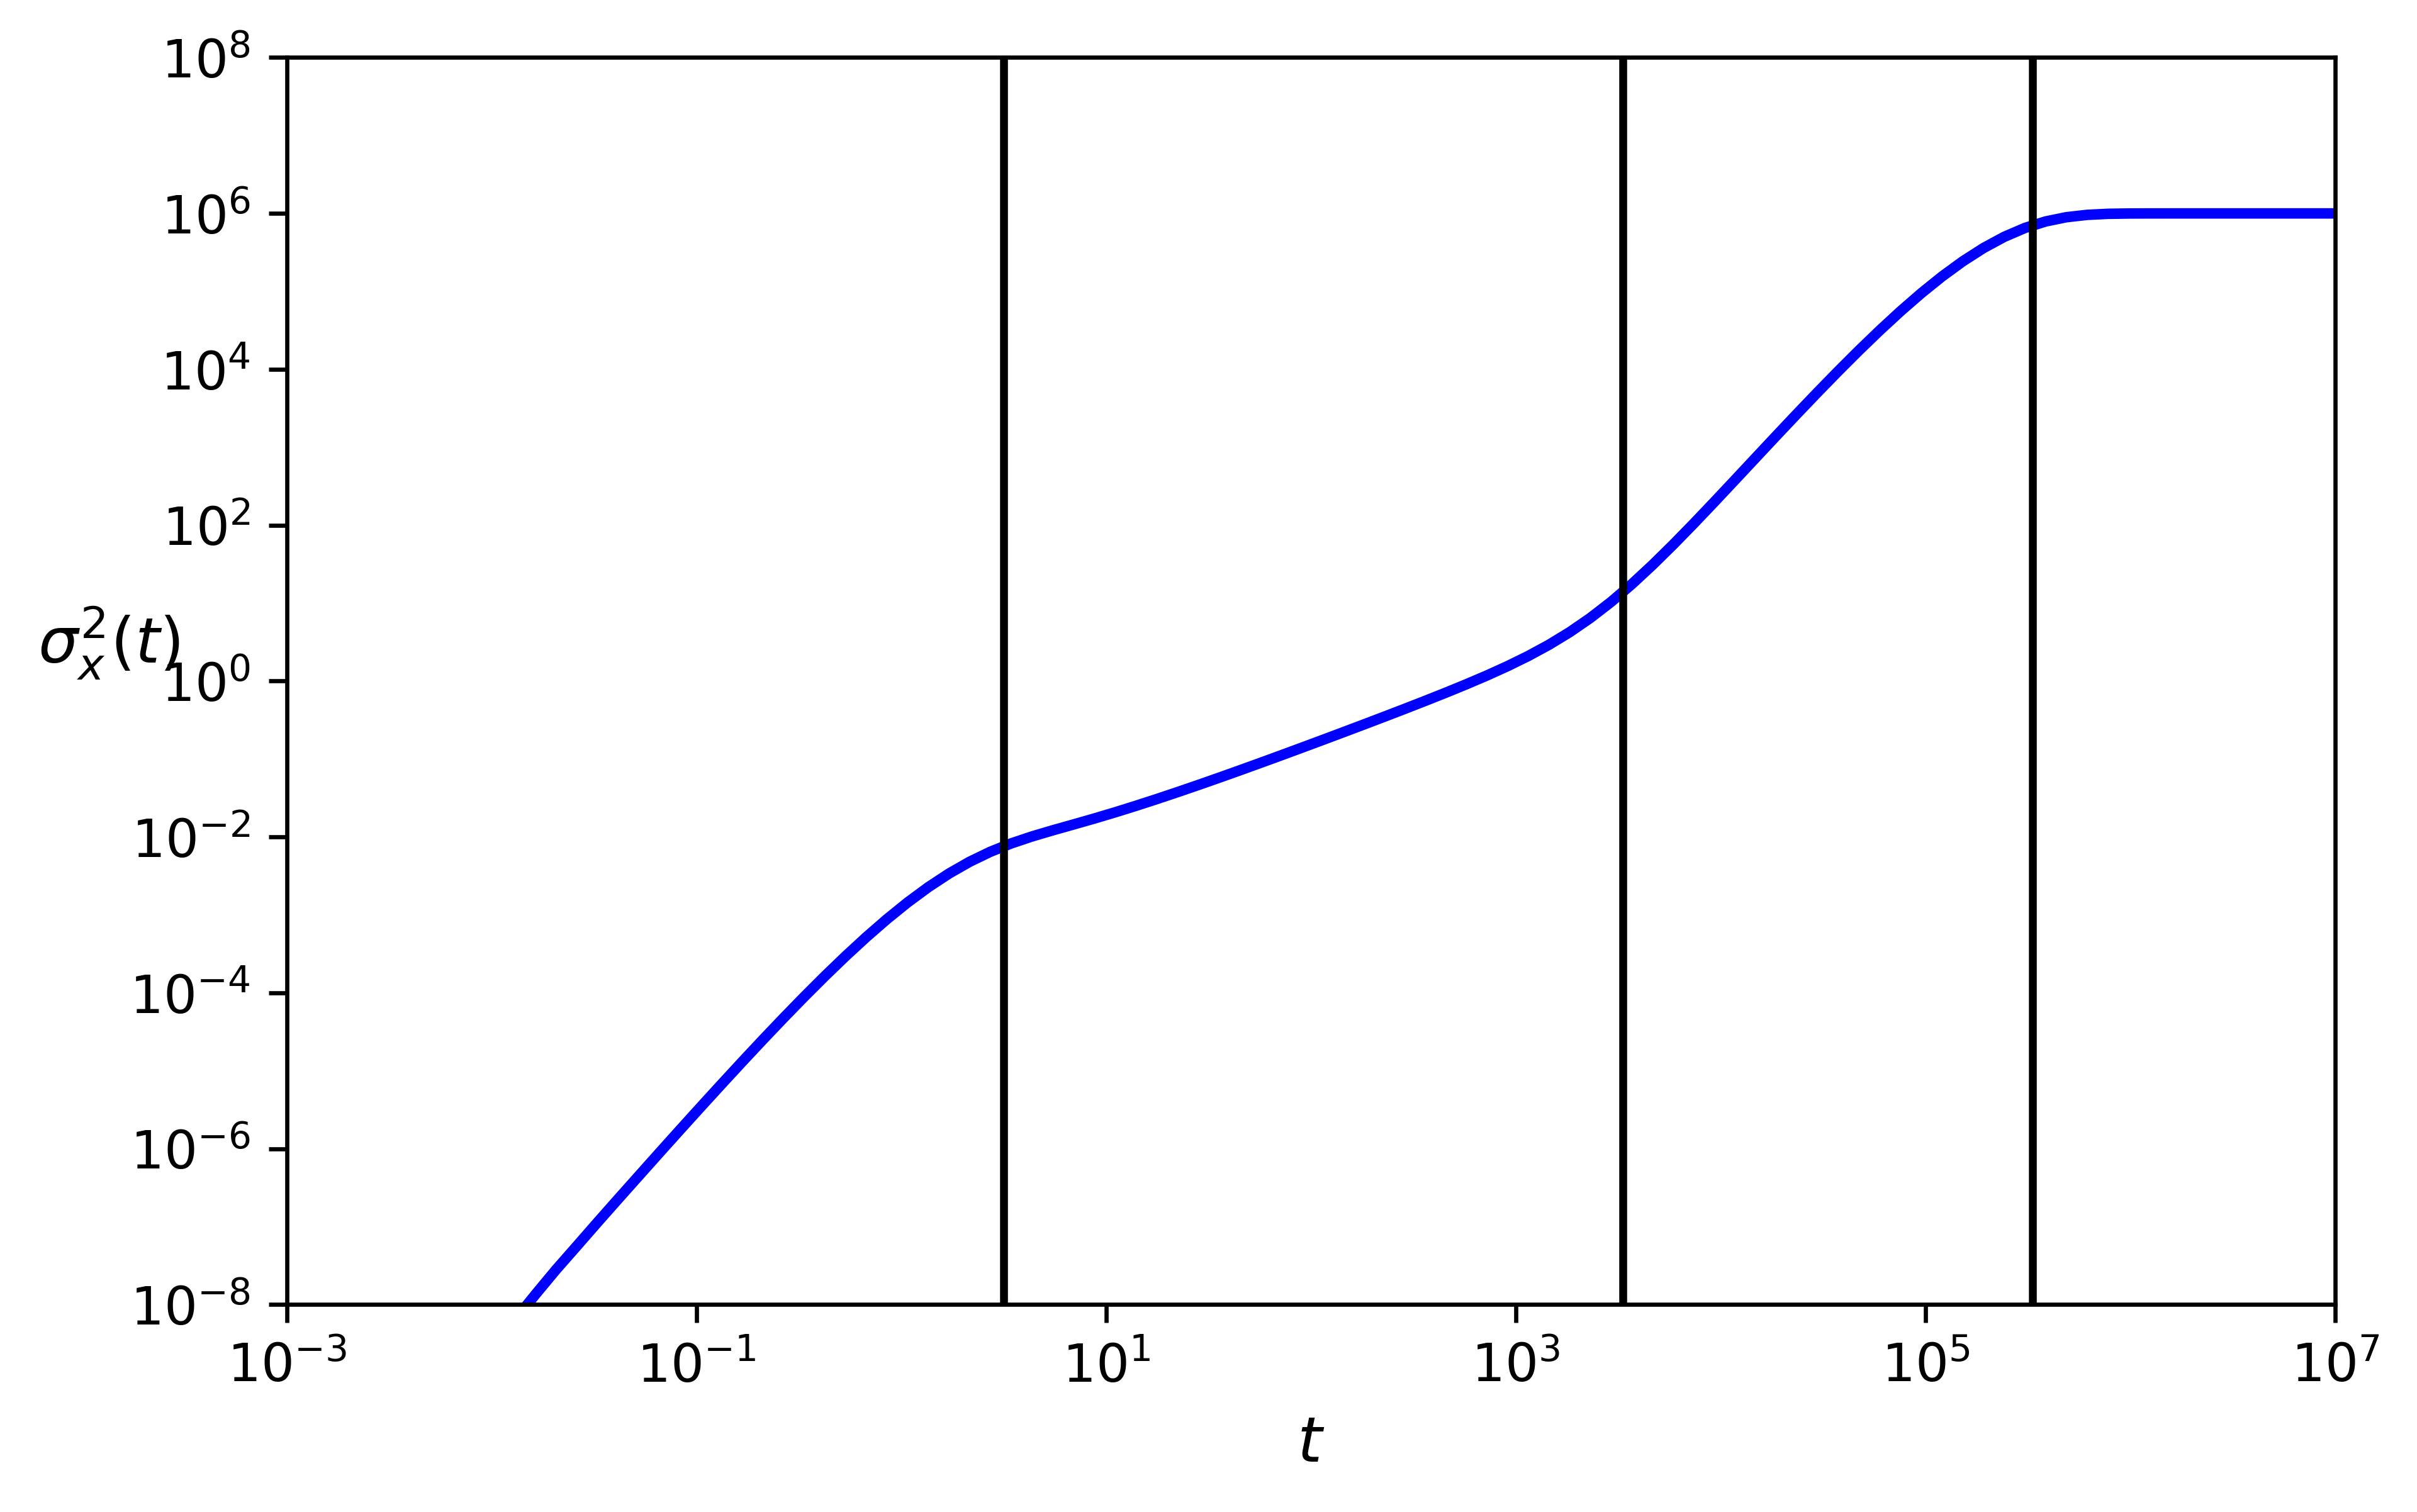
\includegraphics[width=\linewidth,keepaspectratio]{./figures/diffusion.png}
	\caption{The variance of tracer position exhibits four distinct scaling regions as time increases: local, intermediate, global, and finally a non-diffusive range characterized by the eventual trapping of all grains.
	Local and global ranges show super-diffusion $\sigma_x^2 \propto t^3$ while the intermediate range shows normal diffusion. These conclusions hold only for $\kappa \ll k_1 \ll k_2$, meaning motion intervals are generally much shorter than resting intervals, which are in turn are generally much smaller than the time required for resting grains to become buried.}
	\label{fig:var}
\end{figure}
% discuss 3+1 stages of diffusion
For this case there are three stages of diffusion which we associate with the local, intermediate, and global ranges put forth by \citet{Nikora2001a}. There is also a late-stage period of no transport, when the distance between tracers is fixed.
Figure \ref{fig:var} suggests the representation
\be \sigma_x^2 \sim
\begin{cases}
t^{\gamma_\text{local}}, & t\ll \tau_\text{local},\\
t, & \tau_\text{local} \ll t \ll \tau_\text{inter}, \\
t^{\gamma_\text{global}}, & \tau_\text{inter} \ll t \ll \tau_\text{global}, \\
\text{const.}, & \tau_\text{global} \ll  t
\end{cases}\ee
where $\tau_\text{local}$, $\tau_\text{inter}$, and $\tau_\text{global}$ are cross-over times between the diffusion regimes.
$\gamma_\text{local}$ and $\gamma_\text{global}$ are exponents characterizing the local and global range super-diffusion.

% discuss ballistic/normal/ballistic
For the case $1/k_2 \ll 1/k_1 \ll 1/\kappa$ and the initial condition $\theta_1$ the exponents $\gamma_\text{local} \approx 3$ and $\gamma_\text{global} \approx 3$.
% highlight the ranges of cross-over zones and describe physically why
These regions of constant scaling are divided by cross-over zones having finite widths.
Within these zones,the diffusion is not described by a constant scaling law.
The boundaries of these zones are related to the dominant timescales of the transport process.
We identify four key timescales.
These are: (1) the mean time spent in motion, $1/k_2$; (2) the mean time spent at rest, $1/k_1$; (3) the mean time required for a resting grain to trap, $\tau_\text{trap}=1/\kappa$; and (4) the mean time required for a grain switching between motion and rest to trap, $\big(\kappa \frac{k_2}{k_1+k_2}\big)^{-1}$.
To derive the 4th timescale we reason if grain cycles through motion and rest states without trapping, the mean time of a single cycle is $1/k_1 + 1/k_2$, while the mean time spent at rest is $1/k_1$. This means $\frac{1/k_1}{1/k_1 + 1/k_2} = \frac{k_2}{k'}$ is the fraction of time spent at rest \citep[c.f.][]{Ancey2006}. Using this ratio, there is an effective trapping rate $\frac{\kappa k_2}{k'}$ of grains cycling through rest and motion, which supports the 4th characteristic timescale $\frac{k'}{\kappa k_2}$.
The cross-over times $\tau_\text{local}$, $\tau_\text{inter}$, and $\tau_\text{global}$ are geometric means of these four timescales.
We discern $\tau_\text{local} = \sqrt{\frac{1}{k_1}\frac{1}{k_2}}$, $\tau_\text{global} = \sqrt{\frac{1}{\kappa} \frac{k'}{\kappa k_2}}$.
A further geometric mean gives $\tau_\text{inter} = \sqrt{\tau_\text{local}\tau_\text{global}}$.
These timescales are the vertical lines plotted in figure \ref{fig:var}.

% discuss other possibilities
These results pertain to the conditions $1/k_2 \ll 1/k_1 \ll 1/\kappa$ and the initial condition $\theta_1$.
The assumption that rests are much longer than motions was introduced by \citet{Einstein1937}, and it is valid for weak bedload transport that does not resemble a sheet flow \citep{Frey2014}.
We cannot imagine that the characteristic timescale of trapping due to burial $1/\kappa$ would exceed the characteristic resting timescale $1/k_1$, so we consider this constraint always satisfied.
Therefore we need to discern the phenomena of the model for other initial conditions, where $\theta_1 $ and $\theta_2$ are arbitrary; and for the case that $k_1$ and $k_2$ are not well-separated, so that bedload rests are not necessarily much longer than motions.
In these cases, the diffusion characteristics are still described by (\ref{eq:var}), since it is an exact result, but the three-stage diffusion depicted in figure \ref{fig:var} is not necessarily retained.

% effect of initial conditions
The effect of initial conditions on the diffusion phenomena can be surmised using the approach of Tauberian theorems, which are a device to provide small (or large) time asymptotic behavior of a quantity which is known in Laplace space \citep[e.g.][]{Weiss1994}.
We reason that initial conditions cannot affect the intermediate or global range diffusion apart from shifting the $\tau_\text{local}$, since its memory cannot be retained in our model.
We note our model is Markovian by virtue of the choice of exponential propagators \citep{Weiss1994}, meaning it can only have short-term memory.
We show in Appendix \ref{sec:appendixC} that the local range diffusion for arbitrary initial conditions is 
\be \sigma_x^2 \sim v^2 \theta_1 \theta_2 t^2  + \frac{1}{3}(\theta_1 k_1 + \theta_2 k_2)v^2t^3\ee
This is an interesting equation since it encodes a trade-off between $t^2$ and $t^3$ super-diffusion as initial conditions are varied.
If the initial conditions are "pure", meaning all tracers were started at rest or in motion, so one of $\theta_i$ is zero, the local-range diffusion scales as $\sigma_x \sim t^3.$
If the initial conditions are mixed, so both $\theta_i$ are non-zero, diffusion scales as $t^2$, which is still super-diffusive, but with a slower rate of spreading through time.

\subsection{links to earlier works}

% link to lisle 1998
\citet{Lisle1998} generalized the theory of \citet{Einstein1937} to describe the stochastic transport of soil particles under rainfall.
This model includes an exponentially distributed period of motion having velocity $v$ and exponentially distributed resting periods.
Therefore our model is equivalent to that of \citet{Lisle1998} in the limit that the trapping process is turned off: $\kappa \rightarrow 0$.
Taking this limit in (\ref{eq:var}) provides a simpler expression with only two stages of bedload diffusion: a local ballistic range and normal diffusion in the intermediate range. The global range phenomena are not captured since trapping processes are neglected.

% link to Eintsein1937
\citet{Einstein1937} considered steps to be instantaneous, and he characterized them by an exponential step distance distribution.
To access this model from ours, a more careful type of limit is necessary, which reminds one of the limits often used to take continuum limits of lattice theories in physics \citep[e.g.][]{Goldstein1980, Weiss1994}.
This involves sending the mean motion time $1/k_2 \rightarrow 0 $ (equivalent to $k_2 \rightarrow \infty$) while holding the mean step distance $l = v/k_2$ constant.
Denoting the mean resting time by $\tau = 1/k_1$, this results in a bedload variance
\be f=ma \ee
consistent with \citet{Einstein1937}.
This foundational model expresses only single-stage normal diffusion which is associated with the intermediate range. 
The local and global ranges are not captured since the interval of motion and sediment trapping processes are neglected.

% link to Wu2019
More recently, \citet{Wu2019} modeled the diffusion of tracers undergoing burial by assuming grains move in instantaneous steps and may bury with a constant rate while at rest.
Our model includes this in the limit that motions become instantaneous while $\kappa$ is left unconstrained: $k_2 \rightarrow \infty$ as $l = v/k_2$ is held constant and $\kappa \neq 0$.
In this case, (\ref{eq:var}) becomes
\be f=ma \ee
This describes two stages of bedload diffusion as discriminated by \citet{Wu2019}.
There is an intermediate range normal diffusion and a global range super-diffusion.
The local range is not resolved since motion times were neglected.

% discuss limitations and unifying role of this work
Although our model captures three stages of bedload diffusion and unifies a set of earlier works under one mathematical formalism, there are several limitations worth noting.
These constrain its applicability and provide directions for future research.
The major limitation of this work, and, for that matter, the foundational works it builds upon, is that transport characteristics ($k_1, k_2, v, \text{ and }\kappa$, in our case) of sediment grains are considered independent of space and time.
In reality, river channels are often in a state of active adjustment to disturbances in sediment supply regime and variations in hydraulic flow \citep{Church2017}. 
The transport characteristics of individual grains are deeply linked to the morphology of river channels \citep{Hassan2017}, and therefore to morphodynamics as well \citep[e.g.][]{Dhont2018}.
In addition, the (local range) velocities at which grains travel vary from one grain to the next \citep{Fathel2015, Heyman2016} and through time \citep{Fan2014, Ancey2014a} due to turbulence \citep{Celik2014} and the unpredictable nature of bedload collisions with moving \citep{Lee2002} and stationary grains \citep{Gordon1972}.
In summary, bedload transport happens in a spatially and temporally variable environment, so any characteristics of transport necessarily vary in time and space.
To our knowledge, no existing theories have provided a concrete approach to account for this physical problem, and ours is no exception.
To overcome this limitation, is a need to delve deeply into the theory of random phenomena and to applications beyond geophysics.
Surely, there are approaches worth incorporating from other sciences \citep[e.g.][]{Kutner2017}.

\subsection{Geomorphic scaling / scope of conclusions}
% purpose of diffusion understanding
Sediment diffusion in river channels is an important consideration because the motion patterns of individual grains are ultimately responsible for geomorphic change \citep{Hassan2017} and solid contaminant transport through river channels \citep{Malmon2005, Macklin2006}.
This diffusion is anomalous, so any model that describes is also broadly relevant in contemporary science, since anomalous diffusion processes constitute significant difficulties in biology \citep[e.g.][]{Sokolov2012}, geology \citep[e.g.][]{Berkowitz2006}, physics \citep[e.g.][]{Metzler2000}, and chemistry \citep[e.g.][]{Metzler2014}, just as in geomorphology \citep[e.g.][]{Voller2010}.


% issue with linking scales due to scale-dependence of sediment xport
In all of these considerations, the key issue is that anomalous diffusion introduces a scale dependence to the phenomena under study.
In sediment transport, this means the time-scale of observation can affect the measurement of transport characteristics, and descriptions of sediment transport phenomena are necessarily scale dependent.
Indeed, this has been noted in a variety of experiments \citep{Singh2009,Saletti2015,Campagnol2012}.
However, I need to learn more about it to write about it meaningfully.

% we have shown a solution to this deriving all three stages of bedload transport using light-tailed distributions
Although previous authors have derived three-stages of bedload diffusion using models that are equivalent to the inclusion of heavy-tailed sojourn times in a random-walk theory such as ours \citep[e.g.][]{Zhang2012}, and some authors have derived two stages of bedload diffusion \citep[e.g.][]{Wu2019}, we believe we are the first to construct a model of bedload diffusion which encompasses all three stages of bedload diffusion.
We have done this by including trapping processes and finite motion periods into an \citet{Einstein1937}-type model.
In this process, contemporary tools such as the mathematical formalism for continuous time random walks founded by \citet{Montroll1965} and generalized by \citet{Weiss1976} have been essential.


\section{Conclusion}
We have generalized the model of \citet{Einstein1937} to derive the diffusion properties of bedload tracers transporting downstream while undergoing burial.
This reveals three stages of tracer diffusion: an initial superdiffusion $\sigma_x^2 \propto t^2$ or $t^3$ depending on initial conditions, an intermediate normal diffusion $\sigma_x^2 \propto t$, and a late or global range of diffusion $\sigma_x^2 \propto t^\gamma$ with $1\leq \gamma \leq 3$.
These conclusions are a mathematical description of the concepts suggested by \citet{Nikora2001a,Nikora2002}. 
We believe the physical reasoning we've developed here can be used to build new scale-independent descriptions of sediment transport in rivers.
The .
In closing, we believe the legacy of Einstein pervades nearly all contemporary descriptions of sediment transport phenomena, as Einstein was probably the first to take account of the mechanics of individual grains in his descriptions of sediment transport \citep{Einstein1937,Einstein1942,Einstein1950}.
We speculate that geophysical descriptions of phenomena in rivers will become much more sophisticated and  in this century, and this rapid development will be driven by powerful contemporary motivators including climate change \citep{Phillips2016} and the global loss of aquatic biodiversity \citep{Hauer2016}.
Surely this scientific progress would benefit from a careful accounting of its historical foundation.


\appendix

\section{Calculation of the distribution function}
\label{sec:appendixA}
Double transforming (\ref{eq:x}-\ref{eq:y}) using the definition (\ref{eq:doubletransform}) gives
\begin{align}
\tom_{1T}(\eta,s) &= \theta_1 \tg_1(\eta,s) + \tom_2(\eta,s)\tg_1(\eta,s)-\tom_{1F}(\eta,s) \\
\tom_{1F}(\eta,s) &= \theta_1\tg_1(\eta,s+\kappa) + \tom_2(\eta,s)\tg_1(\eta,s+\kappa)\\
\tom_2(\eta,s) &= \theta_2 \tg_2(\eta,s) + \tom_{1F}(\eta,s)\tg_2(\eta,s)
\end{align}
This purely algebraic system solves for 
\begin{align}
\tom_{1T}(\eta,s) &= \frac{\theta_1 + \theta_2 \tg_2(\eta,s)}{1-\tg_1(\eta,s+\kappa)\tg_2(\eta,s)}\big\{\tg_1(\eta,s)-\tg_1(\eta,s+\kappa) \big\} \\
\tom_{1F}(\eta,s) &= \frac{\theta_1 + \theta_2 \tg_2(\eta,s)}{1-\tg_1(\eta,s+\kappa)\tg_2(\eta,s)}\tg_1(\eta,s+\kappa)\\
\tom_{2}(\eta,s) &= \frac{\theta_2 + \theta_1 \tg_1(\eta,s+\kappa)}{1-\tg_1(\eta,s+\kappa)\tg_2(\eta,s)}\tg_2(\eta,s).\\
\end{align}
Double transforming (\ref{eq:b}-\ref{eq:z}) gives
\begin{align}
\tp_0(\eta,s) &= \frac{1}{s}\tom_{1T}(\eta,s)\\
\tp_1(\eta,s) &= \theta_1 \tG_1(\eta,s) + \tom_2(\eta,s) \tG_1(\eta,s) \\
\tp_2(\eta,s) &= \theta_2 \tG_2(\eta,s) + \tom_{1F}(\eta,s)\tG_2(\eta,s).\\
\end{align}
The total probability is $p(x,t) = p_0(x,t) + p_1(x,t) + p_2(x,t)$ or in Laplace space, 
\begin{multline}
\tp(\eta,s) = \frac{1}{s}\frac{\theta_1 + \theta_2 \tg_2(\eta,s)}{1-\tg_1(\eta,s+\kappa)\tg_2(\eta,s)}\big\{\tg_1(\eta,s)-\tg_1(\eta,s+\kappa) \big\} \\
+\frac{\theta_1\big[\tG_1(\eta,s) + \tg_1(\eta,s+\kappa)\tG_2(\eta,s)\big]+ \theta_2\big[\tG_2(\eta,s) + \tg_2(\eta,s)\tG_1(\eta,s)\big]}{1-\tg_1(\eta,s+\kappa)\tg_2(\eta,s)} \\
\label{eq:lap}
\end{multline}
Using the identities $\tg_i(0,s) = \tilde{\psi}_i(s)$ and $\tG_i(0,s) = (1-\tilde{\psi}_i(s))/s$ \citep[e.g.][]{Weiss1994}, it follows that the joint distribution is normalized in space regardless of the choice of propagators: $\tp(0,s) = \mathcal{L}\{\int_0^\infty dx p(x,t);s\} = \mathcal{L}\{1;s\} = 1/s$.
Plugging in the propagators (\ref{eq:prop1}-\ref{eq:prop2}) to \ref{eq:lap} gives 
\be \tilde{p}(\eta,s) = \frac{1}{s}\frac{(s+\kappa + k')s + \kappa k_2 + \theta_1\kappa \eta v}{\eta v(s+\kappa+k_1)+(s+\kappa+k')s + \kappa k_2}.\label{eq:nicedist}\ee
We take the double inverse transform of this equation for the case that grains start in motion.
Setting $\theta_1=0$ and $\theta_2=1$ before inverse transforming (\ref{eq:nicedist}) over $\eta$ first, using the transform 15.103 from \citet{Arfken1985}, provides
\be \tilde{p}(x,s) = \frac{(s+\kappa+k')s+\kappa k_2}{sv(s+\kappa+k_1)}
\exp{\Big(-\frac{s(s+\kappa+k')+\kappa k_2}{s+\kappa+k_1}\frac{x}{v}\Big)}.\ee
Taking the inverse transform over $s$ and leveraging the Laplace transform's linearity, substitution, and translation operations \citep[e.g.][]{Arfken1985} gives the form
\begin{multline}
p(x,t) = e^{-(\kappa + k_1)(t-x/v)-k_2x/v}
\Big[\frac{1}{v}\El^{-1}\Big\{\exp\Big[\frac{k_1k_2}{vs}x\Big];t-x/v\Big\} \\
+ \frac{k_2}{v}\El^{-1}\Big\{\frac{1}{s}\exp\Big[\frac{k_1k_2}{vs}x\Big];t-x/v\Big\} \\
+ \frac{\kappa k_2}{v}\El^{-1}\Big\{\frac{1}{(s-\kappa-k_1)s}\exp\Big[\frac{k_1k_2}{vs}x\Big];t-x/v\Big\}\Big].
\end{multline}
Performing these transforms using entries 2.2.2.1, 2.2.2.8, and 1.1.1.13 from \citet{Prudnikov1992a} and using the definition of the Marcum Q-function \citep[e.g.][]{Temme1996}, we arrive at (\ref{eq:pdf}).

\section{Calculation of the moments}
\label{sec:appendixB}
We employ (\ref{eq:momenttrick}) to compute the moments of position $x$. The first two derivatives of the double Laplace transformed distribution (\ref{eq:lap}) are
\be \partial_\eta \tp(\eta,s) = -v \frac{1}{s}\frac{[(s+\kappa + k')s + \kappa k_2][s+\kappa + k_1]}{[\eta v(s+\kappa +k_1) + (s+ \kappa + k')s+\kappa k_2]^2}\ee
\be \partial_\eta^2 \tp(\eta,s) = 2v^2 \frac{1}{s} \frac{[(s+\kappa + k')s+\kappa k_2][s+\kappa + k_1]^2}{[\eta v(s+\kappa + k_1) + (s+\kappa + k')s+ \kappa k_2]^3}.\ee
Evaluating these at $\eta=0$ and using (\ref{eq:momenttrick}) provides the Laplace transformed moments:
\be  \frac{\bra\tilde{x}(s)\ket} {v} = \Big((\kappa+k_1)s^{-1}+1 \Big)\frac{1}{(s+a)^2-b^2} \label{eq:lapmean}\ee
\be \frac{\bra \tilde{x}^2(s) \ket}{2v^2} = \Big((\kappa+k_1)^2s^{-1} + 2(\kappa+k_1) + s\Big) \frac{1}{[(s+a)^2-b^2]^2}.\label{eq:lapsecondmom}\ee
Where the parameters $a= (\kappa+k')/2$ and $b^2 = a^2 -\kappa k_2$ were introduced to complete the squares in their denominators.
These are inverse transformed by using the linearity and translation properties with those for integration and differentiation \citep[e.g.][]{Arfken1985}.
For the mean this calculation is
\begin{align}
\frac{\bra x \ket}{v} &= \Big((\kappa+k_1)\int_0^t dt \circ+1 \Big)e^{-at}\El^{-1}\Big\{\frac{1}{s^2-b^2};t\Big\}\\
&=  \frac{1}{b}e^{-at}\sinh(bt) + \frac{\kappa + k_1}{2b}\Big[\frac{1}{b-a}\Big(e^{(b-a)t}-1\Big)+ \frac{1}{a+b}\Big(e^{-(a+b)t}-1\Big)\Big]
\end{align}
where the symbol $\circ$ denotes operation on everything to the right of the following parenthesis. In this derivation we used 2.1.5.4 from \citet{Prudnikov1992a}. This equation rearranges to (\ref{eq:mean}).

Applying a similar approach to the second moment (\ref{eq:lapsecondmom}) obtains
\begin{align}
\frac{\bra x^2 \ket}{2v^2} 
&= \Big((\kappa+k_1)^2\int_0^t dt \circ + 2(\kappa + k_1)\circ +  [\partial_t + \delta(t)]\circ \Big)e^{-at}\El^{-1}\Big\{\frac{1}{[s^2-b^2]^2};t\Big\}.\\
\end{align}
Using 2.1.5.6 from \citet{Prudnikov1992a} this becomes
\begin{align}
\frac{\bra x^2 \ket}{2v^2} = \frac{t}{b}\sinh&(bt) + \frac{(\kappa + k_1)}{b^3}\big[bt\cosh(bt)-\sinh(bt)\big]\\
&+e^{-at}\frac{b(b^2(at-2))-a^3t)\cosh(bt) +(a^3-a^2b^2t-3ab^2+b^4t)\sinh(bt)}{(a-b)^2(a+b)^2}
\end{align}
which rearranges to (\ref{eq:second}).
The variance (\ref{eq:var}) follows from $\sigma_x^2 = \bra x^2 \ket - \bra x \ket^2.$

\section{Initial conditions and limiting behaviors}
\label{sec:appendixC}
\subsection{Limit to \citet{Lisle1998}}
The \citet{Lisle1998} model arises from ours in the absence of the trapping process: $\kappa \rightarrow 0$.
In this case, 
\subsection{Limit to \citet{Einstein1937}}
\subsection{Limit to \citet{Wu2019}}
The \citet{Wu2019} model is equivalent to ours when the motions are taken to be instantaneous. This is the limit when $k_2 \rightarrow \infty$ as $l=v/k_2$.
In this case, we discern using Taylor expansions that $b-a \sim -\kappa$, $ a \sim k_2/2$, $b\sim k_2/2$, and $a+b \sim k_2$.
Using these expansions in $A_1$ and $C_1$ from table \ref{table:params} provides
\begin{align}
\frac{A_1}{l} &= -\frac{k_1}{\kappa}\\
\frac{C_1}{l} &= \big(1+\frac{k_1}{\kappa}\big),
\end{align}
meaning the first moment of $x$ is 
\be \frac{\bra x \ket}{l} \sim 1 + \frac{k_1}{\kappa}\big(1-e^{-\kappa t}\big).\ee
Similarly the polynomials involved in the second moment, $A_2$ and $C_2$ limit to 
\begin{align}
\frac{A_2(t)}{l^2} &= -2\frac{k_1}{\kappa} - \Big(\frac{k_1}{\kappa}\Big)^2\big(\kappa t+ 1\big)\\
\frac{C_2}{l^2} &=1+ \Big(\frac{k_1}{\kappa}\Big)^2 + 2\frac{k_1}{\kappa}.\\
\end{align}
We do not require the limiting behavior of $B_1$ and $B_2(t)$ since the exponential factor $\exp(-(a+b)t)$ eliminates these factors in the limit.
These limits provide the second moment as 
\be \frac{\bra x^2 \ket}{l^2} = 1 + 2 \frac{k_1}{\kappa}(1-e^{-\kappa t}) + \Big(\frac{k_1}{\kappa}\Big)^2 (1-(1+\kappa t)e^{-\kappa t}),\ee
meaning the variance in the \citet{Wu2019} limit is 
\be \sigma_x^2 = \Big(\frac{k_1 l}{\kappa}\Big)^2 \Big[(1-\kappa t)e^{-\kappa t}-e^{-2\kappa t}\Big].\label{eq:wuvar}\ee
This equation is similar to the central result of the work by \citet{Wu2019}. It describes two stages of bedload diffusion.
There are minor differences related to the implicit assumption of \citet{Wu2019} that tracers start at rest.
\subsection{Limit to \citet{Wu2019} 2nd attempt}
Our model limits to a close analogue of \citet{Wu2019}.
Taking the limit as $k_2 \rightarrow \infty$ while $v/k_2 = l$ is held constant (the mean step length) and the initial condition is set to $\theta_1=1$ in (\ref{eq:nicedist}) gives
\be\tilde{p}(\eta,s) = \frac{1}{s}\frac{s+\kappa + \kappa l \eta }{\eta l (s + \kappa + k_1) + s + \kappa} .\ee
\citet{Wu2019} assumed a Taylor expansion to second order in the Laplace variable $\eta$ was an appropriate representation of the step length pdf.
In our framework, this transforms the above equation to 
\be \ee



Taking the inverse transform over $\eta$ gives
\be \tilde{p}(x,s) = \frac{1}{s}\Big( [s+\kappa]+\kappa l[\partial_x + \delta(x)]\Big)\frac{1}{l(s+\kappa + k_1)}\exp\Big(- \frac{s+\kappa}{s+\kappa + k_1}\frac{x}{l}\Big)\ee
\acknowledgments
J. Pierce acknowledges a helpful exchange with Eduardo Daly during the early stages of this work. M. Hassan is supported by an NSERC Discovery grant. All simulation code is available on request.

\bibliography{biblio.bib}
\end{document}